%% makeindex these0.nlo -s nomencl.ist -o these0.nls -t these0.nlg

\documentclass[11pt, twoside, openright]{thesis}

%%==============================
% Link to all project .bib
\addbibresource{bib/theory.bib}
\addbibresource{bib/atlas.bib}

%%==============================
% The path to the figures
\graphicspath{{./figures/}}
%%%============================== 
% Include only some chapter for quick compilation
%\includeonly{
%			{tex/abstract},
%}
%%%==============================

\unilogo{figures/university.png}
\lablogo{figures/lal.jpg}
\title{The Thesis full title}
\author{Estelle Scifo}
\university{Université Paris Sud}
\docschool{\'Ecole Doctorale PNC}
\lab{Laboratoire de l'Accélérateur Linéaire}
%\field{Physique des Particules}
\defensedate{11 juillet 2014}
\serienumber{LAL 14-169}

\njurymembers{5}
\addjurymember{1}{M.}{Prénom Nom}{Directeur de thèse}
\addjurymember{2}{Mme.}{Prénom Nom}{Président du jury}
\addjurymember{3}{M.}{Prénom Nom}{Rapporteur}
\addjurymember{4}{Mme.}{Prénom Nom}{Rapporteur}
\addjurymember{5}{M.}{Prénom Nom}{Examinateur}

\begin{document}


%%============================== Titre et sommaires
\frontmatter

\maketitle

\dominitoc % sommaires partiels en début de chapitre


\begin{dedication}
  Some text... 
\end{dedication}


\chapter{Abstract}


\newpage
\hypertarget{contents}{}
\addstarredchapter{Contents}
\tableofcontents

%\printnomenclature
%\mtcfixnomenclature % necessaire pour éviter le decalage des minitoc
%%==============================



%%==============================
%%============================== Corps du texte
%\linenumbers* %%numérotation des lignes à partir de là
\mainmatter

%%-------------------------------
\chapter*{Introduction}
\addstarredchapter{Introduction}



%%-------------------------------
\part{Theory overview}
\chapter{Standard Model}

\chapQuote{A very profound sentence... }{Its author}


\cite{Glashow1961579}

\cite{Salam1964168}

\cite{PhysRevLett.18.507}


%%-------------------------------
\part{Experimental setup and performances}
\chapter{The Large Hadron Collider}

\minitoc\vspace{5ex}


\section{Something... }

\cite{Salam1964168}

\chapter{The ATLAS experiment}
\label{chap:atlas}

\chapQuote{The only way of discovering the limits of the possible is to venture a little way past them into the impossible.}{Clarke's Second Law}

\minitoc\vspace{5ex}

\section*{Introduction}
\addcontentsline{toc}{section}{Introduction}

\section{Physical goals and required performances}
\label{sec:atlas_overview}


\section{Physical constraints and design}
\label{sec:atlas_design}

\section{Detector performances during Run~I}
\label{sec:atlas_performances}

\begin{figure}[h!]\centering
  \subfigure[Integrated luminosity]{\label{fig:lumi_int_dq} 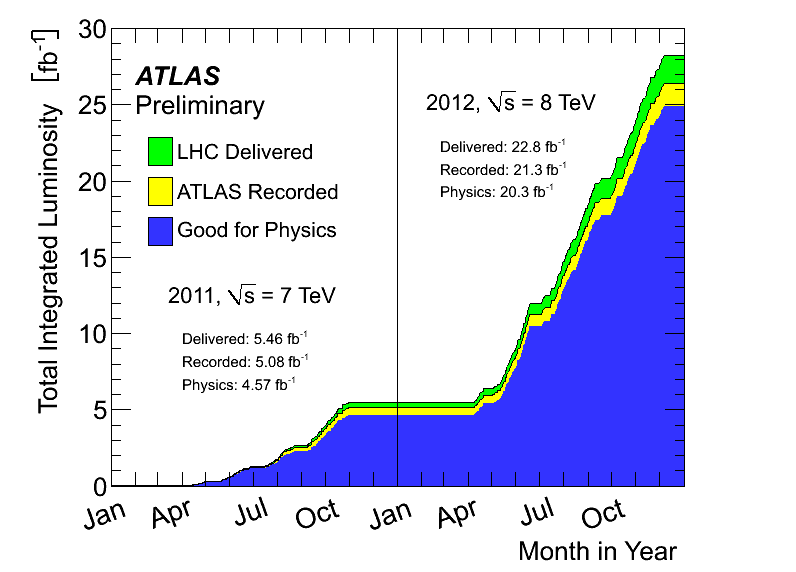
\includegraphics[width=0.48\textwidth]{intlumivstime2011-2012DQ.png}}
  \subfigure[Mean number of interactions per bunch crossing]{\label{fig:mu_2011_20112} 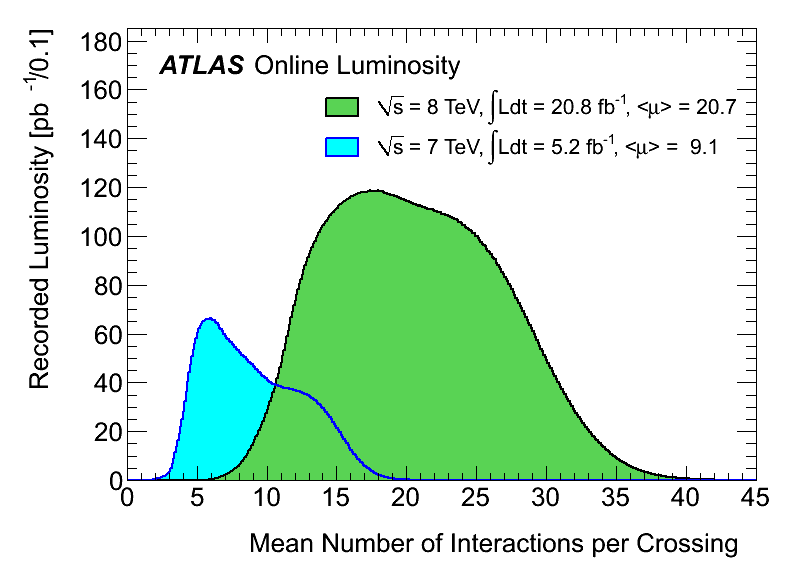
\includegraphics[width=0.48\textwidth]{mu_2011_2012-nov.png}}\\
\caption{(a): luminosity delivered and recorded in ATLAS. (b): mean number of interaction per bunch crossing in 2011 and 2012 data \cite{twiki_lumi}.}
\label{fig:intlumi_atlas}
\end{figure}


%%-------------------------------
\part{Outlooks and conclusion}
\chapter{Conclusion}



%\backmatter
%%==============================
\chapter*{Bibliography}
\addstarredchapter{Bibliography}
\bibbysegment[heading=subbibliography]

%%%==============================
\appendix
\include{tex/appendix}


\backmatter
%%==============================
\include{tex/thanks}



\end{document}
%%==============================
%%==============================
%%==============================
